%!TEX root=..\master.tex
\section{The Bell-LaPadula Security Policy}

In 1973 Bell and LaPadula devised a mathematical model intended for use in  military and governmental computer systems.
The model formalizes users accessing data and how to handle this in a secure way, so confidential information cannot be leaked to a lower classification level.
The following description is based on \citet{lapadula1996secure}.

\subsection{Security}
Before we go into details about how the Bell-LaPadula (BLP) security model is applied to computer systems, we will first discuss some important concepts.

In any system we will have a set of objects $O$ and \subjects{} $S$.
Objects are entities that can somehow be manipulated by \subjects{}.
\Subjects{} are processes or programs in execution that represent a user or a group of users.

\paragraph{Classification and Clearance}
Attached to any object or \ssubject{} will be a classification or clearance respectively.
We denote the set of all classifications/clearances $C = \{C_1, C_2,\dots,C_q\}$ where $\{C_1 > C_2 > \dots > C_q\}$ holds, giving a hierarchical sequence of classifications/clearances.
This means that for any object $o \in O$ with \textit{classification} $C_i \in C$, where $C_i$ is arbitrary, any \ssubject{} $s \in S$ will need a \textit{clearance} $C_j \geq C_i$ in order to access $o$.

\paragraph{Category and Need-to-know}
In addition to classification, objects can belong to one or more categories, which can be seen as security groupings of certain objects.
Similarly, \subjects{} can have one or more need-to-know, which are the security groupings for \subjects{}.
The security categories are a set $K = \{K_1, K_2, \dots, K_r\}$ and unlike classifications/clearances there is no hierarchy of categories.
In order for \ssubject{} $s$ to access an object $o$ with \textit{category} $K_m$ and $K_n$, where $K_m$ and $K_n$ are arbitrary, $s$ must have both \textit{Need-to-know} categories $K_m$ and $K_n$.

\paragraph{Classification and category vectors}
 In the model, classifications and categories are stored in vectors.
 Four functions are used for lookup in these vectors.
 $f_1$ performs a lookup in the \ssubject{} clearance vector, $f_2$ in the object classification vector, $f_3$ in the \ssubject{} need-to-know vector, and finally $f_4$ performs a lookup in the object category function.

\paragraph{Visualization}
This kind of security system can be seen as a \textit{lattice}, see \cref{blp:lattice}.
Each node represents a \emph{security level}, which we define as a combination of classification/clearance and a set of categories.

A \ssubject{} with the clearance \emph{Top Secret} is able to access any object with the security level \emph{Top Secret} and all those below (\emph{Secret} and \emph{Unclassified}).
On the contrary, a \ssubject{} with clearance \emph{Unclassified} can only access objects with the security level \emph{Unclassified}.

Similarly, the category(ies) of each node limit what objects a \ssubject{} can access.
If we have a \ssubject{} $s$ with clearance \emph{Top Secret} and category \emph{Crypto}, $s$ will have access to any objects with security level $(Top Secret, \{Crypto\})$ and those below.

\begin{figure}
\centering
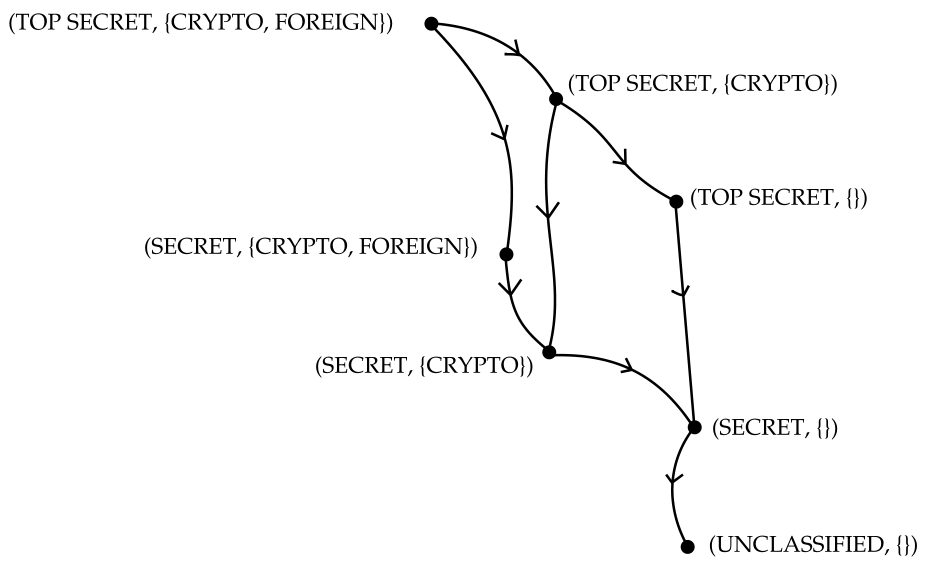
\includegraphics[width=\textwidth]{figures/blp_lattice}
\caption{A BLP lattice \cite{security_engineering_ross_anderson}}
\label{blp:lattice}
\end{figure}

\subsection{Access attributes}\label{blp:access_attributes}
The model considers four attributes for access in a complex computer system: \emph{read-only}, \emph{read/write}, \emph{execute} and \emph{append}.
In addition \emph{control access} is used to give attributes to other users.
Formally, the access attributes are defined as a set in which each member corresponds to the aforementioned attributes:
$$A = \{ r, w, e, a, c \}$$

\paragraph{Read-only}
This attribute makes it possible to read the object but not alter it.
The classical example is a file that contains information that should not be changed.
Alternatively it could be a list containing the \principals{} in the system with their clearance levels.
A \principal{} of low clearance should be able to read this list, but not change it.

\paragraph{Append}
Append describes a pure write operation.
This means that it is possible to append information to the end of a file without being able to extract information about the rest of the file.

This can also be used with a printer which appends information about what is being printed.
By doing this it is sufficient that the classification of a piece of information is matching the classification of the printer in order to prevent unauthorized personnel from reading the information.

\paragraph{Execute}
The execution attribute makes it possible to execute an executable file.
If the \principal{} does not have permission to read from or write to the file he will only be able to execute it.
Similarly, the executable file can produce output that is of a higher classification level than the clearance level of the \principal{} executing it.

\paragraph{Read/write}
This attribute signifies that read and write access are both allowed.
This attribute is what is traditionally used when editing text files.

\paragraph{Control access}
The control access attribute models the notion of a \ssubject{} having control over a file.
Having this attribute a \ssubject{} can give the four attributes above to other \subjects{} in the system.

\subsection{Requests and decisions}
In a computer system the \subjects{} are not directly accessing objects in the system, it is processes in the system that act on behalf of the \ssubject{}.
In the following, a user \emph{requesting} access to a file will be written as a \ssubject{} requesting access and the response to this request a \emph{decision}.

\begin{definition}{Access matrix}\label{blp:def:accessmatrix}
  Let $S$ and $O$ be the \subjects{} and objects (respectively) in a system.
  Then $M$ is an $|O| \times |S|$ matrix representing the current access attributes, and entries $M_{i,j} \subseteq A$ (see \cref{blp:access_attributes}) represent the access attribute that $S_i$ currently has for $O_j$.
\end{definition}

\paragraph{Requests}
There are 4 possible requests that can be made by any \ssubject{}:
\begin{enumerate}
  \item be granted access to an object in a particular mode.
  \item another \ssubject{} should be granted access to an object in a particular mode.
  \item create an object in the system.
  \item delete an object in the system.
\end{enumerate}

In order to carry out the second request, the \ssubject{} needs control access of the object that is being requested access for, as well as the particular mode.
So that for a \ssubject{} $S_i$ requesting read access $r$ for \ssubject{} $S_k$ for object $O_j$, $S_i$ must have both $r$, as well as control access $c$, for $O_j$ itself.
Control access is only given to a certain object when the object is created.
Unlike the other attributes, control access cannot be given by any \ssubject{} to another \ssubject{}.

When a new object is created, it is initially inactive.
In addition to the 4 requests above, in regards to creating objects, we also have the following 2 additional requests:
\begin{enumerate}
  \item alter classification and category assignment of an unused object.
  \item activate an unused object.
\end{enumerate}

For the 4th request, deletion, the object deemed for deletion is inactivated and all current and future privileges are revoked.

\paragraph{Decisions}
Any request made will be met with a response of values $yes$, $no$, $?$, or $error$.
$yes$ and $no$ responses are given when the request is recognized and a check can be performed, thus giving a response of $yes$ if granted and $no$ if not.
$error$ is given in case the request is recognized, but there cannot be given a proper response due to more than a single rule can be applied.
$?$ is given in cases where the request was not recognized.
 
\subsection{Preventing security compromise}\label{bellap:properties}
In order to ensure that data cannot be compromised, the previous definitions of access attributes and requests can be utilized to formalize properties that ensure that compromise cannot occur.

\subsubsection{Security condition}
The security condition states that a \principal{} with a given clearance level is prevented from having read access to any object, which is, or can be, a source of information with a classification level that is higher than the clearance level of the \principal{}.

Formally, this can be expressed as the following:
\begin{definition}{Security condition -- entry}
Let $M_{i,j}$ represent an arbitrary entry in an access matrix, as defined by \cref{blp:def:accessmatrix}.
Then, if and only if
\begin{itemize}
  \item $M_{i,j} \cap \{execute, append, control\} \neq \emptyset$, or
  \item $M_{i,j} \cap \{read, write\} \neq \emptyset \wedge f_1(s) \ge f_2(o) \wedge f_3(s) \supseteq f_4(o)$
\end{itemize}
the entry satisfies the security condition.

\end{definition}
\begin{definition}{Security condition -- system}
An access matrix $M$ satisfies the security condition if
$$\forall S_i \in S: \forall O_j \in O: M_{i,j} \text{ satisfies the security condition}$$

We say that a system is secure if its access matrix satisfies the security condition for all its states.
\end{definition}

Seen in context of the lattice in \cref{blp:lattice}, the security condition can be seen as the disallowance of any \ssubject{} $s$ from reading any objects above its security level.
This is often mentioned in other literature as \emph{no read-up}.

\subsubsection{*-property}
To simplify the description of the *-property we wish to examine which objects a \principal{} has a specific access to.
That is, given a set of attributes $a_1, a_2, \cdots, a_n$, we are interested in the objects that a given \principal{} has either of these access attributes to.
This can be expressed formally as:

\begin{definition}{Matrix extraction}
  Let $S$ represent a \principal{} and $x,y,z \in A$ a set of attributes.
  Then $$b(S:x, y, \cdots, z) = \{o:o\in O \wedge [x \in M_{S,o} \vee y \in M_{S,o} \vee \dots \vee z \in M_{S,o}]\}$$
  represents all the objects to which $S$ has any of the $x, y, \cdots, z$ access attributes.
\end{definition}

The *-property ensures that \principals{} can only write information to an object $o_1$ if that information is read from an object $o_2$ which is at the same or a lower \emph{security level}.
This property must apply to all objects that the principal has access to.

The following definition expresses this formally:
\begin{definition}{*-property}
Let $S$ be a \principal{}.
Then $O_{write} = b(S: w, a)$ is the set of objects to which $S$ can write information and $O_{read} = b(S: r,w)$ the set from which it can read.
Using these sets we can define the *-property for $S$ as:
\begin{align*}
  &\textbf{T} \quad \text{if }O_{write} = \emptyset \vee O_{read} = \emptyset \text{ , otherwise }\\
  &\forall o_w \in O_{write}: \forall o_r \in O_{read}: f_2(o_w) \geq f_2(o_r) \wedge f_4(o_w) \supseteq f_4(o_r)
\end{align*}

\begin{itemize}
  \item A state of an access matrix satisfies the *-property if an only if for each $s \in S$ the following proposition holds.
  \item We say that a system satisfies the *-property if its access matrix satisfies the *-property condition for all its states.
\end{itemize}
\end{definition}

When seeing the *-property in the context of \cref{blp:lattice}, the *-property states that it is not allowed for any \ssubject{} $s$ to read any object $o_1$ and write any of this information to an object $o_2$, if $o_2$ is not above, or at the same security level as, $o_1$.
This is often mentioned as \emph{no write-down}.
